\documentclass[12pt, a4papre]{article}
\usepackage[catalan]{babel}
\usepackage[unicode]{hyperref}
\usepackage{amsmath}
\usepackage{amssymb}
\usepackage{amsthm}
\usepackage{xifthen}
\usepackage{siunitx}
\usepackage{xcolor}
\usepackage{float}
\usepackage{listings}
\usepackage{setspace}
\usepackage{graphicx}
\usepackage{tikz,lipsum,lmodern}
\usepackage[most]{tcolorbox}
\usepackage{circuitikz}
\usepackage{indentfirst}
\usepackage{verbatimbox}
\usepackage[T1]{fontenc}
\usepackage{beramono}% monospaced font with bold variant
 \usepackage{tikz-timing}[2009/05/15]
\usepackage{listings}
\lstdefinelanguage{VHDL}{
   morekeywords={
     library,use,all,entity,is,port,in,out,end,architecture,of,
     begin,and
   },
   morecomment=[l]--
}
 
\usepackage{xcolor}
\colorlet{keyword}{blue!100!black!80}            
\colorlet{comment}{green!50!black!90}
\lstdefinestyle{vhdl}{
   language     = VHDL,
   basicstyle   = \ttfamily,
   keywordstyle = \color{keyword}\bfseries,
   commentstyle = \color{comment}
}

\graphicspath{ {./Imatges/} }


\newcommand{\norm}[1]{\lvert #1 \rvert}

\hypersetup{
    colorlinks = true,
    linkcolor = blue
}

\author{Daniel Vilardell\\
	   Igor Yuziv}
\title{Memoria practica 3}
\date{}

\begin{document}
	\maketitle
	\tableofcontents

	
	\newpage
	\section{Part 1}
	\subsection{Diseny Jerarquic}
	El diseny te l'objectiu de implementar un joc que es basa en endivinar nombres aleatoris amb la informacio de si el nombre entrat es mes gran o mes petit al nombre buscat. Un cop s'endevina s'ha de mostrar el nombre i es pot tornar a començar. Per tal de fer aixo hem creat un programa principal que consta dels seguents components: keygroup, control, comptadorBCD, comparadorBCD i regs\_v. 
	
	Quan es clica una tecla de la placa ho rep keygroup que informa a control si la entrada es un nombre, un asterisc o un coixinet. Control decideix, en funció del moment en que es trobi de la partida(inici, introduccio de dades o final) que fa. En el cas de estar en inici i si s'entra un asterisc el joc comença i es selecciona un nombre aleatori que no es mostra indicant a comptador que pari de contar. Despres si s'entren nombres es van emmagatzemant dins de regs\_v i es van comparant amb el nombre introduit. Nomes quan es clica la tecla coixinet es mostra si el nombre es mes gran o no al buscat.
	
	El component control es l'encarregat de gestionar les fases del joc i decidir que fer en cada moment mentres que comptador es el que decideix el nombre aleatori i comparador retorna si un nombre es mes gran que un altre, i regs de emmagatzemar els nombres introduits.
	
	\newpage
	
	\subsection{ComptadorBCD}
	
	El component comptador es el encarregat de decidir el nombre aleatori. Ho fa de la següent manera: Conte un contador que va augmentant cada flanc de pujada de clk, per tant molt rapidament, i nomes s'atura si ecnt es 0. Com que compta molt rapidament, podem "assegurar" que el nombre escollit sera aleatori. La entrada ecnt la rebrà de control en el moment en que estiguem a fase inicial i es pitgi la tecla asterisc.
	
		\begin{lstlisting}[style=vhdl, frame=single, basicstyle=\tiny]
		library ieee;
use ieee.std_logic_1164.all;
use ieee.std_logic_signed.all;

entity comptadorBCD is
	port (nrst, clk, ecnt : in std_logic;
		numx : out std_logic_vector(7 downto 0));
end comptadorBCD;

architecture compte of comptadorBCD is 
	signal unitats, desenes : std_logic_vector (3 downto 0);
	
begin 
	process(clk, nrst)
	begin
	    if nrst = '0' then desenes <= "0000";
			unitats <= "0000";
	    elsif clk' event and clk='1' then
		if ecnt = '1' then
		if desenes = "1001" and unitats = "1001" then desenes <= "0000";
			unitats <= "0000";
		elsif unitats = "1001" then desenes <= desenes +1;
			unitats <= "0000";
		else unitats <= unitats+1;
		end if;
	    end if;
	end if;
end process;
numx (7 downto 4) <= desenes;
numx (3 downto 0) <= unitats;

end compte;
		
		\end{lstlisting}
		
				
\begin{figure}[H]
		\begin{center}
		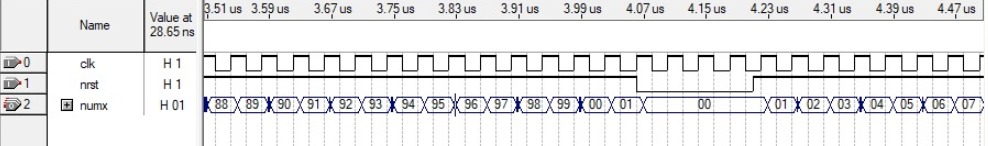
\includegraphics[width=130mm]{simulacioComptador.jpeg}
		\end{center}
	\end{figure}
	
	Podem veure que la simulació ja que quan arriba a 99 torna a començar al 0 i segueix contant.
	
	FALTA CANVIAR SIMULACIO
\begin{figure}[H]
		\begin{center}
		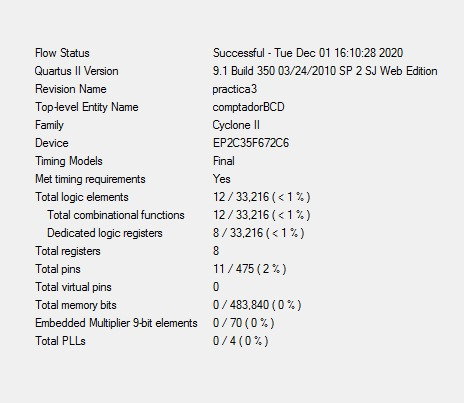
\includegraphics[width=130mm]{informeComptador.jpeg}
		\end{center}
	\end{figure}
	
	
\subsection{ComparadorBCD}

	El bloc comparador també es ben senzill, el que fa es mirar entre dos nombres d'entrada quin es mes gran i donar això a la sortida. Si num > numx aleshores ngtx (n greater than x) serà 1, sin num < numx nltx (n less than x) serà 1 i finalment si son iguals netx(number equal to x) serà 1.
		
	\begin{lstlisting}[style=vhdl, frame=single, basicstyle=\tiny]
	library ieee;
use ieee.std_logic_1164.all;

entity comparadorBCD is 
	port (numx,num : in std_logic_vector (7 downto 0);
			ngtx,nltx,netx: out std_logic);
end comparadorBCD;

architecture comparador of comparadorBCD is 
	begin
	ngtx <= '1' when num > numx else '0';
	netx <= '1' when num = numx else '0';
	nltx <= '1' when num < numx else '0';
end comparador;
	
		\end{lstlisting}

\begin{figure}[H]
		\begin{center}
		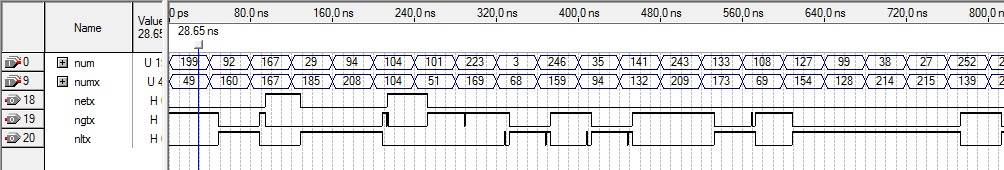
\includegraphics[width=130mm]{simulacioComparador.jpeg}
		\end{center}
\end{figure}

Podem veure que es comporta com hem comentat que faria. En el nostre joc els nombres seran de nomes dos digits, tot i això el component funciona per alguns nombres de 3 digits.



\begin{figure}[H]
		\begin{center}
		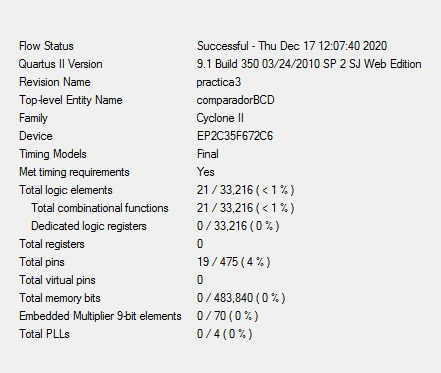
\includegraphics[width=130mm]{informeComparador.jpeg}
		\end{center}
	\end{figure}


\subsection{Control}

	El bloc control es l'encarregat de organitzar les fases del joc i el mes complicat de tots. Aquest bloc conté tres estats. Inicial, Introducció de dades i mostrar resultats. Com a entrades rep si la tecla premuda es un asterisc, un nombre bcd o el coixinet junt amb la relació entre els nombres que s'estan comparant.
	
	\begin{itemize}
		\item \textbf{Inicial:} Per defecte la sortida que indica al contador si seguir contant esta desactivada. Si la entrada es un asterisc indica la atura del comptador posant el bit ecnt a 0 i també canvia l'estat a introduccio de dades.
		\item \textbf{Introducció de dades: }  En aquest estat si la entrada es un nombre bcd, s'indica via la sortida eshft que s'actualitzi el valor del digit dins de regs, on s'emmagatzemen aquests. Si es clica l'asterisc es torna al estat inicial. Si es clica coixinet s'indica a partir de la sortida led i amb la informacio de les entrades ngtx nltx netx si el valor introduit es major, menor o igual i es canvia el estat a mostrar resultats.
		\item \textbf{Mostrar resultats: } En aquest estat control no gestiona res, simplement indica a la sortida eshft que s'han de mostrar els resultats per pantalla (si es major, menor o igual).
	\end{itemize}
		
		\begin{lstlisting}[style=vhdl, frame=single, basicstyle=\tiny]
		
		library ieee;
use ieee.std_logic_1164.all;

entity control is
	port (nrst,clk,bcd,ast,coi,ngtx,netx,nltx : in std_logic;
		ecnt, eshft : out std_logic;
		led : out std_logic_vector(2 downto 0));
	end control;

architecture arcControl of control is 
	type maquina is (inicial, intro_data, mostrar_resultat);
	signal estat: maquina;
begin
	process(clk, nrst) begin
	if nrst = '0' then estat <= inicial;
	elsif (clk'event and clk ='1') then
	    case estat is 
	    when inicial => if ast = '1' then estat <= intro_data; end if;
	    when intro_data => if coi = '1' and ast = '0' then estat <= mostrar_resultat;
			elsif ast = '1' then estat <= inicial; end if;
	    when mostrar_resultat => if ast = '1' then estat <= inicial;
				elsif netx = '1' then estat <= mostrar_resultat;
				elsif bcd = '1' then estat <= intro_data;
				end if;
	    end case;
	end if;
end process;

ecnt <= '1' when estat = inicial else '0';
eshft <= '1' when (estat = intro_data or estat = mostrar_resultat) and bcd = '1' else '0';
			
led <= "111" when estat = inicial 
    else "100" when estat = mostrar_resultat and nltx = '1' 
        and netx= '0' and ngtx = '0'
    else "010" when estat = mostrar_resultat and netx = '1' 
    	and nltx = '0' and ngtx = '0'
    else "001" when estat = mostrar_resultat and ngtx = '1' 
    	and nltx = '0' and netx = '0'
    else "000";
end arcControl;
		
		\end{lstlisting}
		
		FALTA SIMULACIO CONTROL

	
	
	\begin{figure}[H]
		\begin{center}
		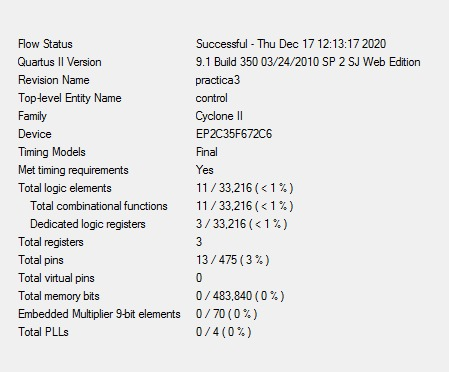
\includegraphics[width=130mm]{informeControl.jpeg}
		\end{center}
	\end{figure}	
		
		
\subsection{Registres}

	Registres funciona igual que a la ultima practica, es un mòdul seqüencial síncron que te com a finalitat carregar i memoritzar els digits introduits opA i opB. Aquest, si la entrada intro es 1 i clk esta en el flanc de pujada i nrst esta activat, actualitzara els valors de opA i opB, posant a opA el valor entrat per keycode i a opB el antic valor de opA.
	
		\begin{lstlisting}[style=vhdl, frame=single, basicstyle=\tiny]

library ieee;
use ieee.std_logic_1164.all;

entity regs_v is
	port(clk, nrst, intro : in std_logic;
		 keycode : in std_logic_vector(3 downto 0);
		 opA, opB: out std_logic_vector(3 downto 0));
end regs_v;

architecture arq of regs_v is
signal a, b : std_logic_vector(3 downto 0);
begin
process (clk, nrst)
begin 
	if(nrst = '0') then a <= "0000"; b <= "0000";
	elsif(nrst='1') and (clk'event and clk = '1') and (intro = '1') then
			b <= a;
			a <= keycode;
	end if;
end process;
opA <= a;
opB <= b;

end arq;

		\end{lstlisting}
		
			\begin{figure}[H]
		\begin{center}
		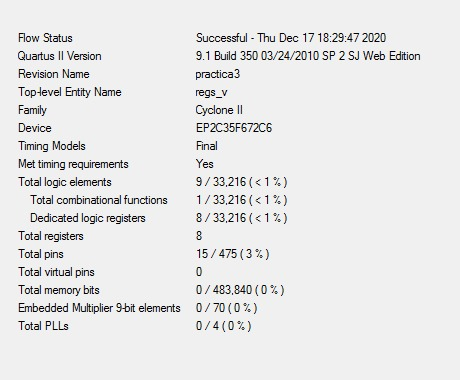
\includegraphics[width=130mm]{informeRegs.jpeg}
		\end{center}
	\end{figure}	


\subsection{keygroup}

	Aquest component també es igual a la practica anterior i te com a finalitat indicarnos si la tecla premuda es un nombre bcd, un asterisc o un coixinet.
	
		\begin{lstlisting}[style=vhdl, frame=single, basicstyle=\tiny]
	library ieee;
use ieee.std_logic_1164.all;

entity keygroup_v is
	port(nkey : in std_logic;
		k : in std_logic_vector(3 downto 0);
		bcd, ast, coi : out std_logic);
end keygroup_v;

architecture arq of keygroup_v is
begin
process (nkey, k)
begin
	if (nkey = '0' and (k = "0000" or k = "0001" or k = "0010" or
				k = "0011" or k = "0100" or k = "0101" or
				k = "0110" or k = "0111" or k = "1000" or
				k = "1001")) then bcd <= '1'; ast <= '0'; coi <= '0';
	elsif(nkey = '0' and k = "1110")
			then bcd <= '0'; ast <= '1'; coi <= '0';
	elsif(nkey = '0' and k = "1111")
			then bcd <= '0'; ast <= '0'; coi <= '1';
	elsif(nkey = '1') then bcd <= '0'; ast <= '0'; coi <= '0';
	end if;
end process;
end arq;
		\end{lstlisting}
		
			\begin{figure}[H]
		\begin{center}
		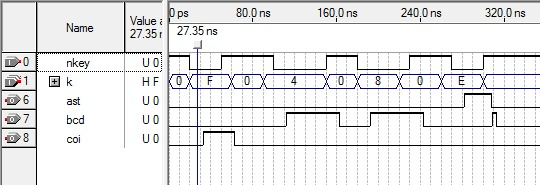
\includegraphics[width=130mm]{simulaciokeygroup.jpeg}
		\end{center}
	\end{figure}	
	Veiem que funciona ja que s'activa coi quan la entrada es F, bcd quan la entrada es 4 i 8 i ast quan la entrada es E.
	
	
			\begin{figure}[H]
		\begin{center}
		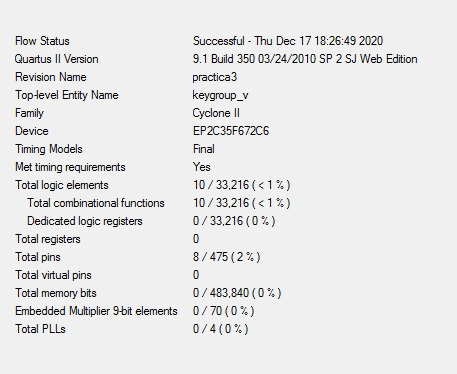
\includegraphics[width=130mm]{informeKeygroup.jpeg}
		\end{center}
	\end{figure}	
	
	\subsection{Leds}
	
	El component Leds transforma 3 bits a 8 bits .
	
		\begin{lstlisting}[style=vhdl, frame=single, basicstyle=\tiny]
		
	library ieee;
use ieee.std_logic_1164.all;

entity leds is
	port(led: in std_logic_vector(2 downto 0);
		 led_green : out std_logic_vector(7 downto 0));
end leds;

architecture arq of leds is
begin
	led_green <= "11111111" when led = "111" else
				 "11110000" when led = "100" else
				 "00001111" when led = "001" else
				 "00111100" when led = "010" else
				 "00000000" when led = "000";
				 
end arq;

		\end{lstlisting}
		
		
			\begin{figure}[H]
		\begin{center}
		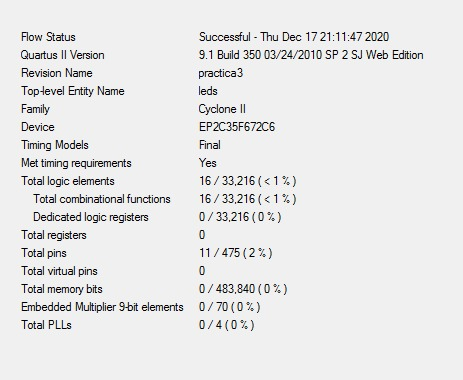
\includegraphics[width=130mm]{informeLeds1.jpeg}
		\end{center}
	\end{figure}
	
	\subsection{Joc}
	Aquest es el programa principal breument explicat al inici de la practica. Consta de tots els components mencionats anteriorment i els ajunta per a controlar la part principal del joc. La entrada es passa per keygroup que ens diu quin tipus d'entrada es, que s'envia a control. En funció de en quin estat control es trobi aturara el contador, mostrara si el valor introduit es mes gran o igual o mes petit o actialitzarà el valor de regs. Com a entrades rebrà si s'esta clicant una tecla, quina tecla s'esta pitjant, nrst i clk. Com a sortida indicarà quins leds iluminar junt amb el nombre introduit per l'usuari.
	
				\begin{figure}[H]
		\begin{center}
		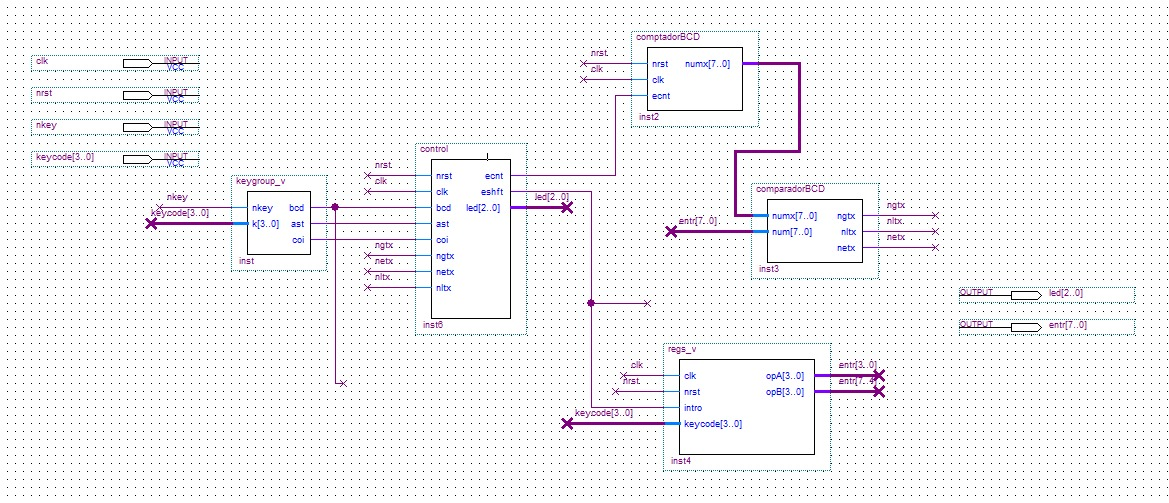
\includegraphics[width=130mm]{joc.jpeg}
		\end{center}
	\end{figure}	
			\begin{figure}[H]
		\begin{center}
		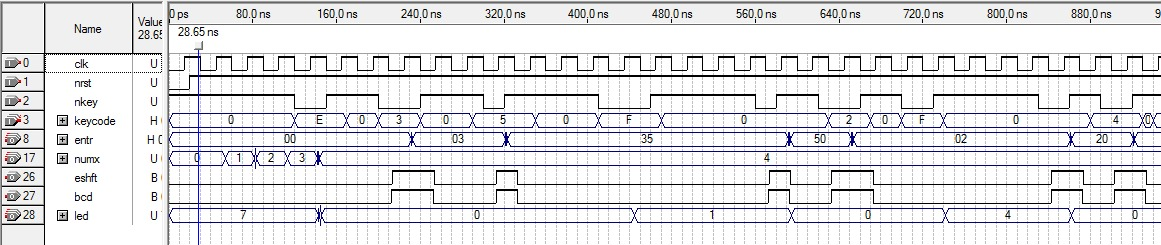
\includegraphics[width=130mm]{simulacioJoc.jpeg}
		\end{center}
	\end{figure}	
			\begin{figure}[H]
		\begin{center}
		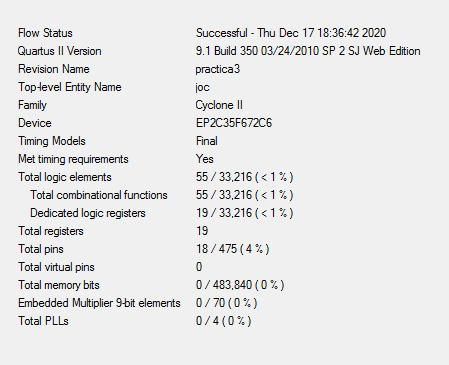
\includegraphics[width=130mm]{informeJoc.jpeg}
		\end{center}
	\end{figure}	

		
	\subsection{Joc Placa}
	
	Un cop ja hem testejat tots els components individualment amb simulacións ho ajuntem tot a un diagrama de blocs amb l'objectiu de mostrarho i interectuar a la placa. 
	
	Aquest diagrama funciona de la seguent manera, keytest s'encarrega de indicar quina tecla s'està prement i la introdueix al programa principal indicat anteriorment. Aquest ens indicara el nombre entrat per l'usuari a mostrar per la sortida entr i els leds a iluminar led. El component leds que s'encarregara de transformar la sortida led de 3 bits a una sortida de 7 que indicarà els leds a iluminar. El component hex\_disp transforma els nombres de la entrada a 7 segments per a mostrar a la placa els valors.
	
	\begin{figure}[H]
		\begin{center}
		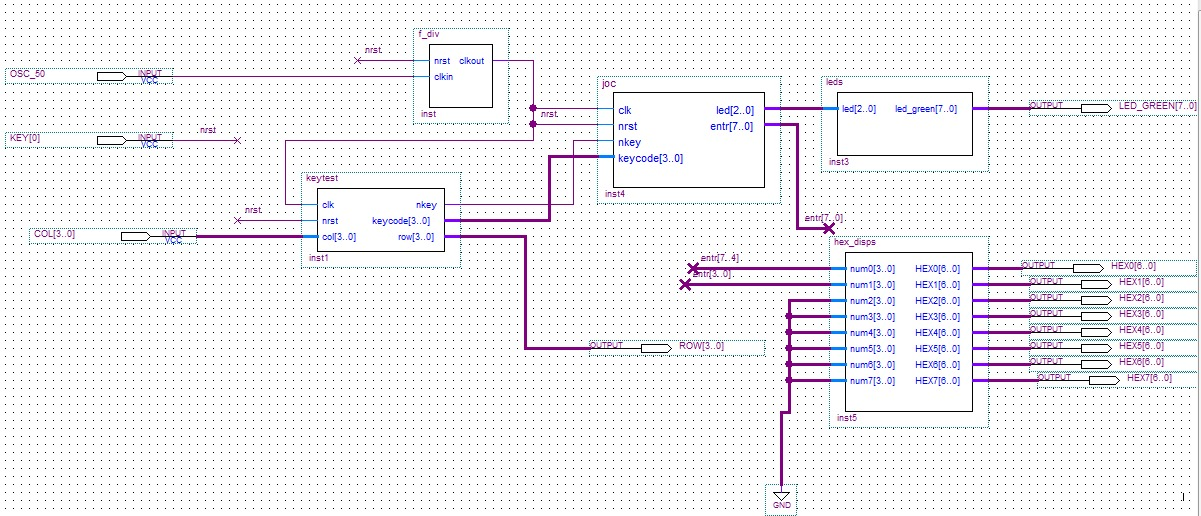
\includegraphics[width=130mm]{jocPlaca.jpeg}
		\end{center}
	\end{figure}	

\newpage

\section{Part Extra}

Un cop tenim el joc basic hem decidit ampliarlo de la seguent forma. Primer hem introduit un altre digit al joc, es a dir, en contes d'adivinar un nombre de 2 digits s'ha d'endivinar un nombre de 3. Com que això podria arribar a ser aburrit hem havilitat una forma de fer trampes: pitjant la tecla B es pot veure el valor de les desenes del nombre buscat i la tecla A per a veure les unitats. Aixi doncs nomes faltaria un  nombre per a adivinar, el de les centenes. 
A mes d'això hem havilitat un sistema que fa un conta enrere i un contador de punts a base de leds per tal de competir a contrarellotge i intentar fer els maxims punts en un temps donat.

Per a fer aquesta part hem hagut de fer moltes modificacions a la primera part del progecte, algunes d'aquestes son les seguents. Hem modificat contador per a que conti fins a les centenes

\subsection{ComptadorBCD Extra}

	\begin{lstlisting}[style=vhdl, frame=single, basicstyle=\tiny]

library ieee;
use ieee.std_logic_1164.all;
use ieee.std_logic_signed.all;

entity comptadorBCD_extra is
	port (nrst, clk, ecnt : in std_logic;
		numx : out std_logic_vector(11 downto 0));
end comptadorBCD_extra;

architecture compte of comptadorBCD_extra is 
	signal unitats, desenes, centenes : std_logic_vector (3 downto 0);
	
begin 
	process(clk, nrst)
	begin
	    if nrst = '0' then desenes <= "0000";
			unitats <= "0000"; centenes <= "0000";
	    elsif clk' event and clk='1' then
		if ecnt = '1' then
		if desenes = "1001" and unitats = "1001" and centenes = "1001" 
			then desenes <= "0000"; unitats <= "0000"; centenes <= "0000";
		elsif desenes = "1001" and unitats = "1001" then centenes <= centenes + 1;
			desenes <= "0000"; unitats <= "0000";
		elsif unitats = "1001" then desenes <= desenes + 1;
			unitats <= "0000";
		else unitats <= unitats+1;
		end if;
	    end if;
	end if;
end process;
numx (11 downto 8) <= centenes;
numx (7 downto 4) <= desenes;
numx (3 downto 0) <= unitats;

end compte;

		\end{lstlisting}
		
				\begin{figure}[H]
		\begin{center}
		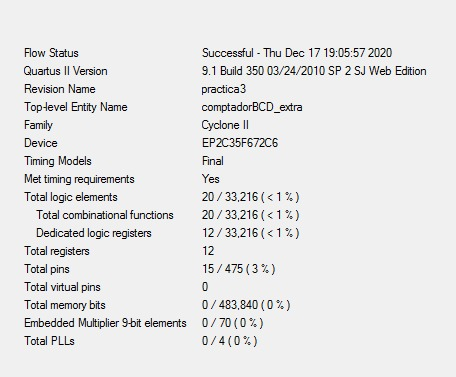
\includegraphics[width=130mm]{informeComptadorBCDextra.jpeg}
		\end{center}
	\end{figure}	
		

\subsection{Registres Extra}

	\begin{lstlisting}[style=vhdl, frame=single, basicstyle=\tiny]
	library ieee;
use ieee.std_logic_1164.all;

entity regs_extra is
	port(clk, nrst, intro : in std_logic;
		 keycode : in std_logic_vector(3 downto 0);
		 opA, opB, opC: out std_logic_vector(3 downto 0));
end regs_extra;

architecture arq of regs_extra is
signal a, b, c : std_logic_vector(3 downto 0);
begin
process (clk, nrst)
begin 
	if(nrst = '0') then a <= "0000"; b <= "0000"; c <= "0000";
	elsif(nrst='1') and (clk'event and clk = '1') and (intro = '1') then
			c <= b;
			b <= a;
			a <= keycode;
	end if;
end process;
opA <= a;
opB <= b;
opC <= c;

end arq;
	
			\end{lstlisting}
			
						\begin{figure}[H]
		\begin{center}
		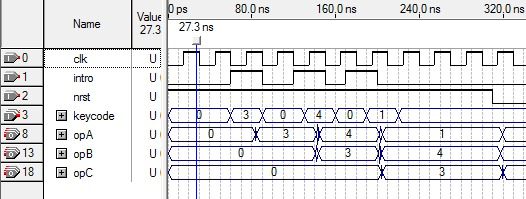
\includegraphics[width=130mm]{simularioRegistreExtra.jpeg}
		\end{center}
	\end{figure}	
	
					\begin{figure}[H]
		\begin{center}
		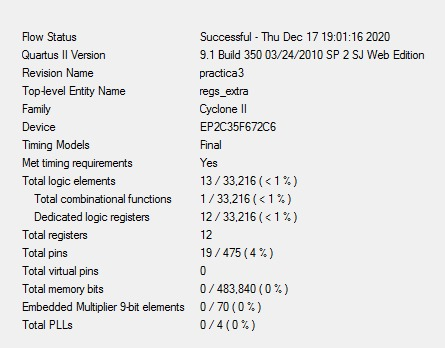
\includegraphics[width=130mm]{informeRegsExtra.jpeg}
		\end{center}
	\end{figure}	
	
			
			

\subsection{Keygroup Extra}


	\begin{lstlisting}[style=vhdl, frame=single, basicstyle=\tiny]

library ieee;
use ieee.std_logic_1164.all;

entity keygroup_extra is
	port(nkey : in std_logic;
		k : in std_logic_vector(3 downto 0);
		bcd, ast, coi, A, B : out std_logic);
end keygroup_extra;

architecture arq of keygroup_extra is
begin
process (nkey, k)
begin
	if (nkey = '0' and (k = "0000" or k = "0001" or k = "0010" or
						k = "0011" or k = "0100" or k = "0101" or
						k = "0110" or k = "0111" or k = "1000" or
						k = "1001")) then bcd <= '1'; ast <= '0'; coi <= '0'; A <= '0'; B <= '0';
	elsif(nkey = '0' and k = "1010") then bcd <= '0'; ast <= '0'; coi <= '0'; A <= '1'; B <= '0';
	elsif(nkey = '0' and k = "1011") then bcd <= '0'; ast <= '0'; coi <= '0'; A <= '0'; B <= '1';
	elsif(nkey = '0' and k = "1110") then bcd <= '0'; ast <= '1'; coi <= '0'; A <= '0'; B <= '0';
	elsif(nkey = '0' and k = "1111") then bcd <= '0'; ast <= '0'; coi <= '1'; A <= '0'; B <= '0';
	elsif(nkey = '1') then bcd <= '0'; ast <= '0'; coi <= '0'; A <= '0'; B <= '0';
	else bcd <= '0'; ast <= '0'; coi <= '0'; A <= '0'; B <= '0';
	end if;
end process;
end arq;


			\end{lstlisting}
			
			
						\begin{figure}[H]
		\begin{center}
		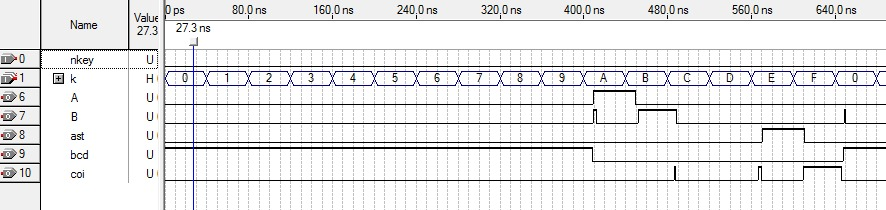
\includegraphics[width=130mm]{simulacioKeyGroupExtra.jpeg}
		\end{center}
	\end{figure}	
		\begin{figure}[H]
			
				\begin{center}
		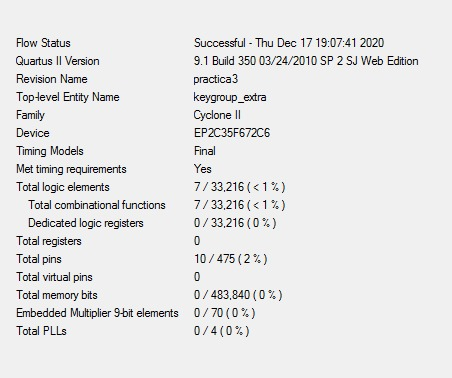
\includegraphics[width=130mm]{informeKeyGroupExtra.jpeg}
		\end{center}
	\end{figure}	
			
			
\subsection{Control Extra}

	\begin{lstlisting}[style=vhdl, frame=single, basicstyle=\tiny]

library ieee;
use ieee.std_logic_1164.all;
use ieee.std_logic_unsigned.all;

entity control_extra is
	port (nrst,clk,bcd,ast,coi,A,B,ngtx,netx,nltx : in std_logic;
		ecnt, eshft : out std_logic;
		led : out std_logic_vector(2 downto 0);
		tot : out std_logic_vector(3 downto 0));
	end control_extra;

architecture arcControl of control_extra is 
	type maquina is (inicial, intro_data, mostrar_resultat, trampa_A, trampa_B);
	signal estat: maquina;
	signal t : std_logic_vector(3 downto 0);
begin
	process(clk, nrst) begin
	if nrst = '0' then estat <= inicial;
	elsif (clk'event and clk ='1') then
	    case estat is 
	    when inicial => if ast = '1' then estat <= intro_data; end if;
	    when intro_data => if coi = '1' and ast = '0' then estat <= mostrar_resultat;
						   elsif ast = '1' then estat <= inicial;
						   elsif A = '1' then estat <= trampa_A;
						   elsif B = '1' then estat <= trampa_B; end if;
	    when mostrar_resultat => if ast = '1' then estat <= inicial;
				elsif bcd = '1' then estat <= intro_data;
				elsif A = '1' then estat <= trampa_A;
				elsif B = '1' then estat <= trampa_B;
				end if;
		when trampa_A => if ast = '1' then estat <= inicial;
				elsif bcd = '1' then estat <= intro_data;
				elsif B = '1' then estat <= trampa_B;
				end if;
		when trampa_B => if ast = '1' then estat <= inicial;
				elsif bcd = '1' then estat <= intro_data;
				elsif A = '1' then estat <= trampa_A;
				end if;
		end case;
		if(netx = '1' and estat = intro_data) then t <= t + 1; estat <= inicial; end if;
	end if;
end process;
tot <= t;

ecnt <= '1' when estat = inicial else '0';
eshft <= '1' when (estat = intro_data or estat = mostrar_resultat) and bcd = '1' else '0';
			
led <= "111" when estat = inicial 
    else "100" when estat = mostrar_resultat and nltx = '1' 
        and netx= '0' and ngtx = '0'
    else "010" when estat = mostrar_resultat and netx = '1' 
    	and nltx = '0' and ngtx = '0'
    else "001" when estat = mostrar_resultat and ngtx = '1' 
    	and nltx = '0' and netx = '0'
    else "110" when estat = trampa_A
    else "011" when estat = trampa_B
    else "000";
end arcControl;

			\end{lstlisting}
			
			
			
				\begin{figure}[H]
			
				\begin{center}
		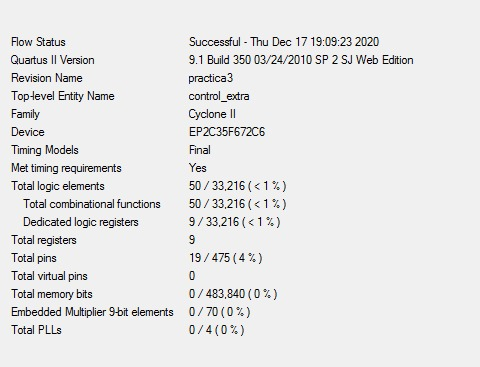
\includegraphics[width=130mm]{informeControlExtra.jpeg}
		\end{center}
	\end{figure}	
			
\subsection{Trampes}
	\begin{lstlisting}[style=vhdl, frame=single, basicstyle=\tiny]

library ieee;
use ieee.std_logic_1164.all;

entity trampes is
	port(tr : in std_logic_vector(2 downto 0);
		 num: in std_logic_vector(11 downto 0);
		 mostra: out std_logic_vector(3 downto 0));
end trampes;

architecture arq of trampes is
begin
process (tr)
begin
	if tr = "110" then mostra <= num(3 downto 0);
	elsif tr = "011" then mostra <= num(7 downto 4);
	else mostra <= "0000";
	end if;
end process;
end arq;



			\end{lstlisting}
			
			\begin{figure}[H]
			
				\begin{center}
		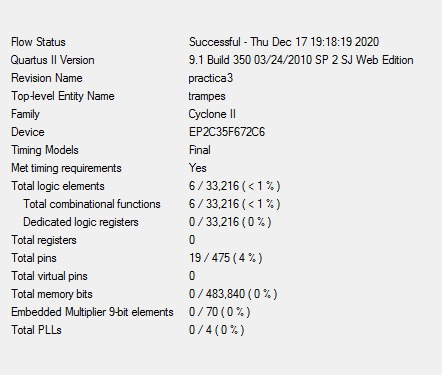
\includegraphics[width=130mm]{informeTrampes.jpeg}
		\end{center}
	\end{figure}	

			
			
\subsection{Leds Extra}

	\begin{lstlisting}[style=vhdl, frame=single, basicstyle=\tiny]
	library ieee;
use ieee.std_logic_1164.all;

entity led_extra is
	port(led: in std_logic_vector(2 downto 0);
		 num : in std_logic_vector(3 downto 0);
		 led_green : out std_logic_vector(7 downto 0);
		 led_level : out std_logic_vector(7 downto 0));
end led_extra;

architecture arq of led_extra is
begin
	led_green <= "11111111" when led = "111" else
				 "11110000" when led = "100" else
				 "00001111" when led = "001" else
				 "00111100" when led = "010" else
				 "00000000" when led = "000" else
				 "01010101" when led = "110" else
				 "10101010" when led = "011";
	led_level <= "00000000" when num = "0000" else
				 "10000000" when num = "0001" else
				 "11000000" when num = "0010" else
				 "11100000" when num = "0011" else
				 "11110000" when num = "0100" else
				 "11111000" when num = "0101" else
				 "11111100" when num = "0110" else
				 "11111110" when num = "0111" else
				 "11111111" when num = "1000";
				 
end arq;
	\end{lstlisting}
	

	
			\begin{figure}[H]
			
				\begin{center}
		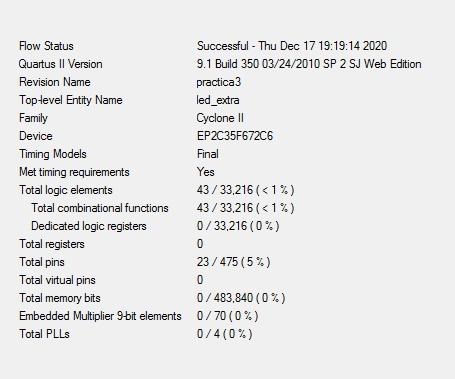
\includegraphics[width=130mm]{informeLeds.jpeg}
		\end{center}
	\end{figure}
	
\subsection{Temporitzador}


\begin{lstlisting}[style=vhdl, frame=single, basicstyle=\tiny]
	library ieee;
use ieee.std_logic_1164.all;
use ieee.std_logic_signed.all;

entity temporitzador is
	port (nrst, clk, ecnt : in std_logic;
		numx : out std_logic_vector(7 downto 0));
end temporitzador;

architecture compte of temporitzador is 
	signal unitats, desenes : std_logic_vector (3 downto 0);
	
begin 
	process(clk, nrst)
	begin
	    if nrst = '0' then desenes <= "1001";
			unitats <= "1001";
	    elsif clk' event and clk='1' then
		if ecnt = '1' then
		if desenes = "0000" and unitats = "0000" then desenes <= "0000";
			unitats <= "0000";
		elsif unitats = "0000" then desenes <= desenes -1;
			unitats <= "1001";
		else unitats <= unitats-1;
		end if;
	    end if;
	end if;
end process;
numx (7 downto 4) <= desenes;
numx (3 downto 0) <= unitats;

end compte;
	\end{lstlisting}
	
	
			\begin{figure}[H]
			
				\begin{center}
		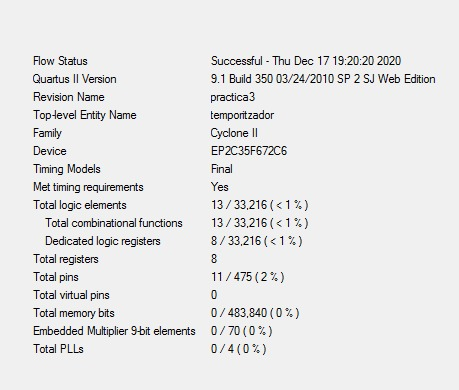
\includegraphics[width=130mm]{informeTemporitzador.jpeg}
		\end{center}
	\end{figure}
	
	
\subsection{Slow Timer}
\begin{lstlisting}[style=vhdl, frame=single, basicstyle=\tiny]
	-- Frequency divider by M
-- D = output duty cycle in %
-- version DD-1.0 - march 2011

library ieee;
use ieee.std_logic_1164.all;

entity slow_timer is 
  port( nrst,clkin : in std_logic; 
        clkout : out std_logic );
end slow_timer;

architecture dni of slow_timer is
constant M : integer :=750;
constant D : integer :=50;
constant n : integer :=D*M/100;
signal q : integer range 0 to M-1;
begin
  process(clkin,nrst) begin
     if nrst='0' then clkout <= '0'; q <= 0;
     elsif clkin'event and clkin='1' then 
         if q < M-1 then q <= q+1; 
            else q <= 0; end if;
         if q < n then clkout <= '1';
            else clkout <= '0'; end if;
     end if;
  end process;
end dni;
	\end{lstlisting}
	

	
		\begin{figure}[H]
			
				\begin{center}
		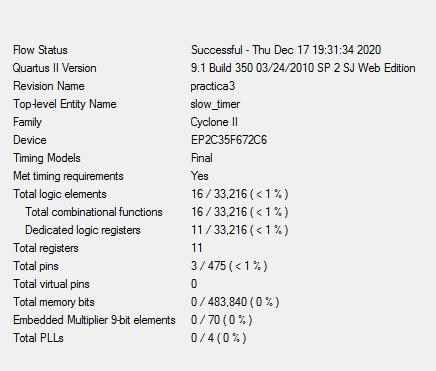
\includegraphics[width=130mm]{informeSlowTimer.jpeg}
		\end{center}
	\end{figure}
\subsection{Joc Extra}


\begin{figure}[H]
			
				\begin{center}
		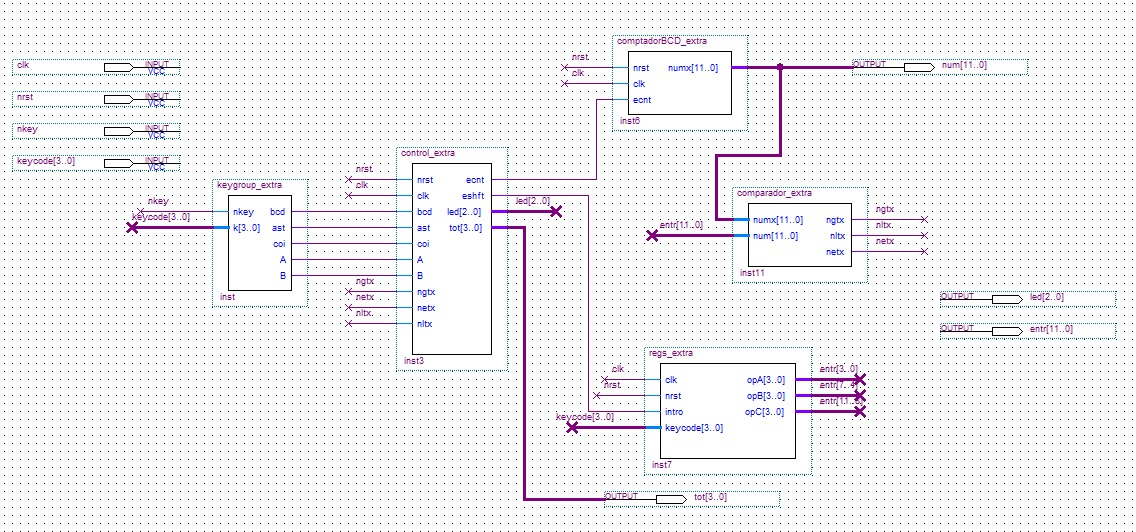
\includegraphics[width=130mm]{jocExtra.jpeg}
		\end{center}
	\end{figure}
	
	\begin{figure}[H]
	
				\begin{center}
		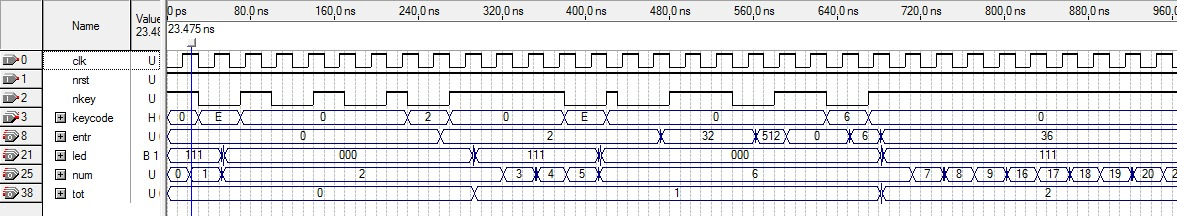
\includegraphics[width=130mm]{SimulacioJocExtra.jpeg}
		\end{center}
	\end{figure}
	
	
	\begin{figure}[H]
	
				\begin{center}
		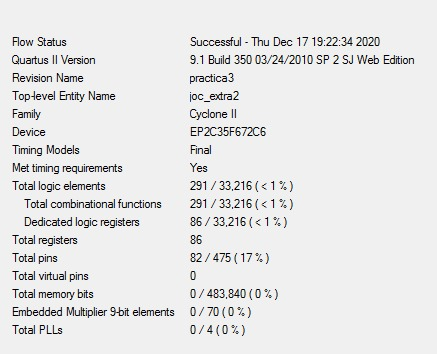
\includegraphics[width=130mm]{informeJocExtra.jpeg}
		\end{center}
	\end{figure}
	

\subsection{Joc Extra Placa}

	\begin{figure}[H]
	
				\begin{center}
		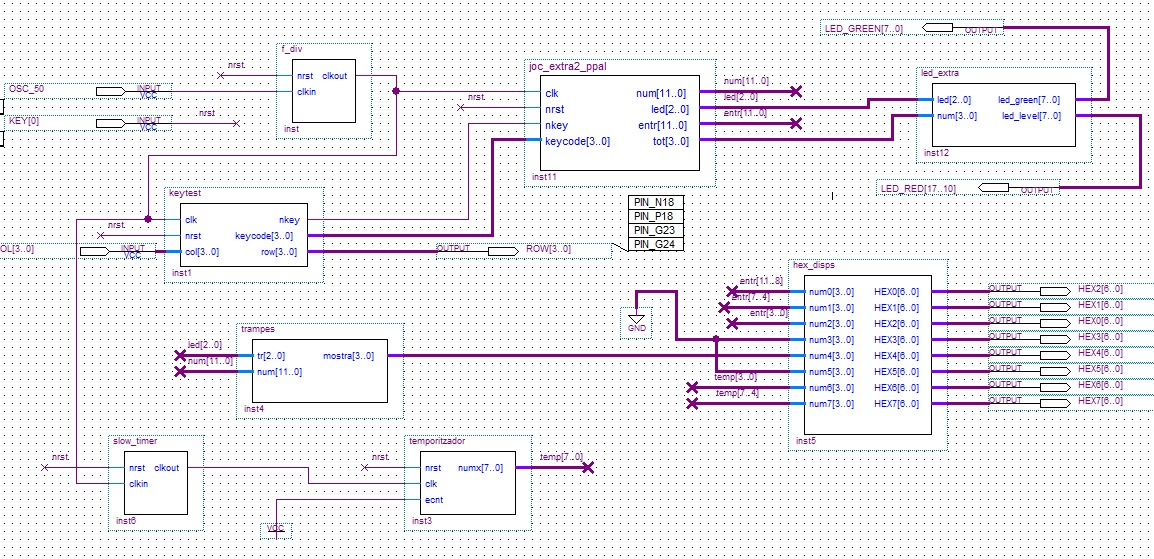
\includegraphics[width=130mm]{JocExtraPlaca.jpeg}
		\end{center}
	\end{figure}
	
	
\end{document}